\chapter{Literature Review}

Current adult image filtering techniques can be classified into three categories: keyword based, blacklist based and content based. Our proposed system is content based i.e. images will be classified on the basis of their content. The classification approach we applied can be broadly classified into two categories- Skin based and non-skin based.

%
\section{Skin Based Approach}
Our human civilization has been influenced and intoxicated by the web revolution. People of every age use the web for different needs and purposes. Some use it for fun; some use it for their studies and find information while some live on it. Images are essentially part of the modern web and we all agree to the fact that a single picture is worth thousand words. We can find all sort of information on the web and it has been a part of our daily life. However, it also has abundance of images and contents that may be unsuitable for certain age groups. Finding pornographic images posted on social sites and links on study groups is not a new thing in today’s world. Pornographic images certainly need to be managed and unavailable to children and men at work.  

\subsection{Skin Color Detection Method}
The most important feature that provides clues to image content is color. Color is a low level feature, which makes it computationally inexpensive and therefore suitable for real-time object characterization, detection and localization. Generally pornographic images show a lot of skin and thus skin color is a basic feature used in detecting pornographic images. The main goal of skin color detection or classification is to build a decision rule that will discriminate between skin and non-skin pixels. Identifying skin colored pixels involves finding the range of values for which most skin pixels would fall in a given color space


\subsubsection{Color Spaces}
The purpose of a color space is to facilitate the specification of colors in some standard, generally accepted manner. A color space is a specification of a coordinate system and subspace within a system where each color is represented by a single point. Various color spaces are used for processing digital images. For some purposes, one color space may be more appropriate than others.  

\subsubsection{The RGB Color Space}
The RGB color space originated from CRT display applications.  In the RGB space each color appears in its primary spectral component of red, green, and blue.  Images represented in the RGB space consist of three component images, one for each primary color.  When fed into an RGB monitor, these images combine on the phosphor screen to produce a composite  color image (Gonzalez and Woods, 2002).The RGB color space is one of the most widely used color spaces for storing and processing digital image.  However, the RGB color space alone is not reliable for identifying skin-colored pixels since it represents not only color but also luminance.  Skin luminance may vary within and across persons due to ambient lighting so it is not dependable for segmenting skin and non-skin regions.   Chromatic colors are more reliable and these are obtained by eliminating luminance through some form of transformation.  The color spaces Normalized RGB, HSV, and YCbCr are transformations commonly used by studies on skin color (Waibel et al., 1999).


\subsubsection{The HSV Color Space}
The HSV (Hue, Saturation, Value/Intensity/Luminance) color space describes color with intuitive values, based on the artist’s idea of tint, saturation and tone.  This was introduced when there was a need to specify color properties numerically.  Hue defines the dominant color as described by wavelength, for instance the distinction between red and yellow.   Saturation measures the colorfulness of an area in proportion to its brightness such as the distinction between red and pink.   Value refers to the color luminance, the distinction between a dark red and a light  red. For skin detection, the value component is discarded to eliminate the undesirable effect of uneven illumination.  The transformation is defined by

\begin{align}
H&=\arccos\frac{\frac{1}{2} (R-G)+ (R-B)}{\sqrt{(R-G)^2 + (R-B)(G-B)}}\\
S&=1-\frac{3min(R,G,B)}{R+G+B}\\
V&=\frac{R+G+ B}{3}
\end{align}

Some studies show that HSV is invariant to highlights at white light sources, to matte surfaces, and ambient lighting. However, hue discontinuities and the computation of the luminance component conflict badly with the properties of color vision.

\subsubsection{The YCbCr Color Spacr}
YCbCr or Y′CbCr is a family of color spaces used as a part of the color image pipeline in video and digital photography systems. Y′ is the luma component and CB and CR are the blue-difference and red-difference chroma  components. Y' (with prime) is distinguished from Y which is luminance, meaning that light intensity is non-linearly encoded using gamma.

Y'CbCr is not an absolute color space, it is a way of encoding RGB information. The actual color displayed depends on the actual RGB colorants used to display the signal. Therefore a value expressed as Y′CbCr is only predictable if standard RGB colorants or an ICC profile are used.The transformation from RGB to YCbCr is defined by
\begin{align}
Y'&=16+ (65.481R + 128.553G + 24.966B)\\
Cb&=128+(-37.797R- 74.203G +112B)\\
Cr&=128+(112R -93.786G - 18.214B)
\end{align}
%

\section {Non Skin Based Approach}


\subsection {BIC}
\clearpage
\subsection {MPEG-7}



The MPEG-7 standard\cite{Mpeg} is an international standard since September 2001
which specifies metadata for describing multimedia content. The interest-
ing part for our project is this part of the standard which defines visual
descriptors. These are structures to describe multimedia data. Their exact
extraction methods are not standardized.  shows an overview of
MPEG-7 visual descriptors which are suitable for still images.
Since 2001, lots of research has been conducted on making use of these
standardized visual descriptors in the field of Computer Vision, especially in
Content-Based Image Retrieval Systems 
\begin{figure}[h]
  \centering
  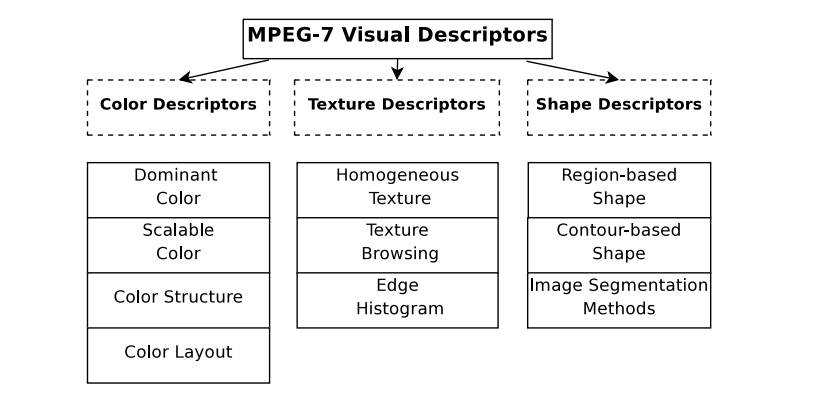
\includegraphics[width=6in]{Mpeg7}
  \caption  {MPEG-7 Visual Descriptors For Low-level Features.}
   \label{Mpeg7}
\end{figure}


\subsubsection {Dominant ColorDescriptor}
Dominant Color Descriptor  (DCD) provides an effective, 
compact  and  intuitive  description  of  the  representative 
colors  in  an  image or  region  . The descriptor  consists 
of  the  Color  Index  (ci),  Percentage  (pi),  Color Variance 
(vi) and Spatial Coherency (s); the last two parameters are 
optional.  Then the DCD is defined by: 
\begin{align}
F={(c_{i},p_{i},v_{i}),s}, i=1,....,N
\end{align} 
where N is the number of the colors and                      . 
For dominant  color  extraction,  the  generalized Lloyd 
algorithm  is  used  for  color  clustering. 
There is one overall Spatial Coherency (SC) value for the 
whole  image  and  several  groups  of $(c_{i},  p_{i},  v_{i}) $  for  the 
corresponding dominant colors. The  Perceptual  colors  to  represent  images  based  on  dominant colors  \ref{DCD}
\begin{table}[h]
\begin{tabular}{| c | c | c |c |}
\hline
S/No.              & Red &Green &Blue   \\
\hline
Manchester United & 6 & 4 & 0   \\
Celtic            & 6 & 3 & 0    \\
FC Porto           & 6 & 2 & 1   \\
FC Copenhagen     & 6 & 2 & 1  \\
\end{tabular}
\caption{ Perceptual  colors  to  represent  images  based  on  dominant colors }
  \label{DCD}

\end{table}
\subsubsection{DCD Extraction}
The  extraction  procedure  for  the dominant  color  uses  the Generalized Lloyd Algorithm (GLA)\cite{vector}  to  cluster  the  pixel  color  values. After  defining  the  colors,  for  each  image implement the following steps:
\begin{itemize}
\item Read  in  the  image  and  create  an  image  array  that 
contains  the RGB components of each pixel  in  the 
image
\item For each pixel in the image do: 
	\begin{itemize}
	\item Search  color  table  for  the  nearest  color  by finding  the distance between  the pixel  color  I 
		represented as  $(P_{r}, P_{g}, P_{b})$ and  the color  in  the color  table $ C_{i}$  represented  as 
		$(C_{iR},  C_{iG},  C_{iB})$ using the distance formula (3): 
		\[  C_{d}=(\sqrt{(P_{r}-C_{ir})^2 + (P_{g}-C_{ig})^2 + (P_{b}-C_{ib})^2}), \]
                        \qquad  i=1,2....18
	\item Assign  to  the  pixel  the  RGB  entry  in  color table for which $C_{d}$ is the minimum
	\end{itemize}
\item Create a frequency table for each assigned color 
\item Sort  the  frequency  table  in  descending  order MPEG-7  DCD  allows  at  most  eight  colors  to  be 
	represented.The  highest  four  frequent colors  are  then  selected  with  their  percentages  to 
	create the description of the image.
\end{itemize}


\subsubsection{Edge Histogram Descriptor}
The EHD represents the spatial distribution of edges in an image. The extraction process of the EHD consists of the following stages:
\begin{itemize}
\item The edges in each image-block is categorized into one of the following
	six types: vertical, horizontal, 45◦
diagonal, 135◦
diagonal, nondirectional edge and no-edge. (See Figure 8)
\item Now a 5-bin edge histogram of each subimage can be obtained. (See \ref{ehd})
\item Each bin value is normalized by the total number of image-blocks in the image.
\item The normalized bin values are nonlinearly quantized.
\begin{figure}[htp]

     \subfigure [Horizontal Edge]{\label{ehd-a} \includegraphics[scale=0.60]{{horizontal}}}
   \qquad \subfigure[Vertical Edge]{\label{ehd-b}
\includegraphics[scale=0.6]{vertical}} 
  \qquad    \subfigure[45 degree edge ]{\label{ehd-c}
\includegraphics[scale=0.6]{diagonal}} \\ 
	\subfigure [135 degree edge] {\label{ehd-d}
\includegraphics[scale=0.6]{135}}
\qquad \subfigure [non-directional edge] {\label{ehd-e}
\includegraphics[scale=0.6]{no-direction}}

  \caption{Five types of Edges}
  \label{ehd}
\end{figure}
\end{itemize}


\subsection {Edge and Moment Appraoch}

\subsubsection{Edge Detection}
An edge in an image is a contour across which the brightness of the image changes abruptly.
In image processing, an edge is often interpreted as one class of singularities. In a function,
singularities can be characterized easily as discontinuities where the gradient approaches
infinity. However, image data is discrete, so edges in an image often are defined as the
local maxima of the gradient.
\\
Edge detection is an important task in image processing. It is a main tool in pattern
recognition, image segmentation, and scene analysis. An edge detector is basically a high-
pass filter that can be applied to extract the edge points in an image.

\subsubsection{Classical Edge Detectors}
Many classical edge detectors have been developed over time. They are based on the
principle of matching local image segments withspecificedgepatterns. Theedgedetection
is realized by the convolution with a set of directional derivative masks.The popular edge detection operators are Roberts, Sobel, Prewitt, Frei-Chen, and Laplacian operators
Creating a footnote is easy.\footnote{An example footnote.}  	an example footnote.
\subsubsection{Sobel Edge Detector}

\[
G_{x}=
 \begin{bmatrix}
  +1 &+2 &+1 \\
  0 & 0 & 0 \\
  -1 & -2 & -1
 \end{bmatrix} *A
\]
\[
G_{y}=
 \begin{bmatrix}
  +1 & 0 & -1 \\
  +2 & 0 & -2 \\
  +1 & 0 & -1
 \end{bmatrix}
\]

\subsubsection {Multiscale Edge Detector}
The resolution of an image is directly related to the proper scale for edge detection. High
resolution and small scale will result in noisy and discontinuous edges; low resolution and
large scale will result in undetected edges.Because image data is always discrete, the practical scale in images is usually integer.
\\
The scale controls the significance of edges to be shown. Edges of higher significance
aremorelikelytobekeptbythewavelettransformacross scales. Edges of lower significance
are more likely to disappear when the scale increases.

\subsubsection {Image Moments}
Spatial and central moments are important statistical properties of an image.An image moment is a certain particular weighted average (moment) of the image pixels' intensities, or a function of such moments, usually chosen to have some attractive property or interpretation.
Image moments are useful to describe objects after segmentation. Simple properties of the image which are found via image moments include area (or total intensity), its centroid, and information about its orientation.

\par
For a 2-D moment of order (p+q) of a digital image f(x,y) is defined as

\begin{align}  m_{pq}=  \sum_{x} \sum_{y} x^p y^q f(x,y)  \end{align}
 
for p,q=0,1,2,....., where the summations are over the values of the spatial coordinates x and y spanning the image. The corresponding \emph{central moment} is defined as 
\begin{align} \mu_{pq} = \sum_{x} \sum_{y} (x-\bar{x})^p (y-\bar{y})^q f(x,y) \end{align}
where \[ \bar{x}=\frac{m_{10}}{m_{00}} \quad and \quad \bar{y}=\frac{m_{01}}{m_{00}} \]

\par
The \emph{normalized central moment} of order (p+q) is defined as 
\[  \eta_{pq}=\frac{\mu_{pq}} {\mu_{00}^\gamma} \]
for p,q=0,1,2,...., where 
\[ \gamma=\frac {p+q} {2} +1  \]
for p+q=2,3,.....

\par
A set of seven 2-D \emph{moment invariants} that are insensitive to translation,scale change , mirroring and rotation can be derived from these equations. They are

\begin{align}
&\phi_{1}=\eta_{20} + \eta_{02} \\
&\phi_{2}=(\eta_{20} -eta_{02})^2 + 4\eta_{11}^2   \\
&\phi_{3}=(\eta_{30} -3\eta_{12})^2 + (3\eta_{21}-\eta_{03})^2  \\ 
&\phi_{4}=(\eta_{30} + \eta_{12})^2 + (\eta_{21} + \eta_{03})^2  &\\
&\phi_{5}=(\eta_{30}-3\eta_{12})(\eta_{30} + \eta_{12})  \nonumber \\
		 &\qquad [(\eta_{30}+\eta_{12})^2  - 3(\eta_{21} + \eta_{03})^2 ] + \nonumber \\
		& \qquad(3\eta_{21}-\eta_{03}  (\eta_{21}+\eta_{03}) \nonumber \\		
		&\qquad[3(\eta_{30}+\eta_{12})^2 - (\eta_{21}+\eta_{03}^2]  \\
&\phi_{6}=(\eta_{20}-\eta_{02})[(\eta_{30}+\eta_{12}^2 -(\eta_{21}+\eta_{03})^2] \nonumber\\
	&\qquad+ 4\eta_{11}(\eta_{30}+\eta_{12})(\eta_21 + \eta_{03})  \\
&\phi_{7}=(3\eta_{21} -\eta_{03})(\eta_{30}+\eta_{12})[ (\eta_{30} + \eta_{12})^2 \nonumber \\
		&\qquad-3(\eta_{21}+ \eta_{03})^2] + (e\eta_{12}=\eta_{30})(\eta_{21}+\eta_{03})\nonumber \\
		&\qquad[3(\eta_{30}+\eta_{12})^2 - (\eta_{21} + \eta_{03})^2]
\end{align}
These sets of equations are commonly referred as Hu set of invariant moments.\cite{hu62}

\subsubsection {Procedure}
Multiscale Edge detection since sobel is just not good enough
Process is started with the multiscale edge detection . Once the edge image is computed. we compute the normalized central moments upto order five and the translation,rotation and scale invariant based on the grayscale edge image using the definitions.A feature vector containing these 21+7=28 moments is computed and stored in the training database.\cite{Wang97}

\section {SVM(Support Vector Machine)}
The  central  idea  of SVM  is  the  adjustment  of  a  discriminating  function  so  that  it  optimally  uses  the  separability information of the boundary cases. Given a set of cases which belong  to one of  two classes,  training a  linear SVM consists  in  searching  for  the hyperplane  that  leaves  the  largest possible number of  cases  of  the  same  class  on  the same side, while maximizing the distance of either class from the hyperplane. If the training set is linearly separable, then a discriminant hyperplane will satisfy the inequalities:
\begin{equation}
v_{i}(w.x_{i}+b) \geq 1
\end{equation}

 where $x_{i}$  $\in$  $\Re^d$ is a  vector  of  the  training  set,  d  being  the  dimension  of  the  input  space,  and $y_{i}$  $\in$ ${\{-1,+1\}}$ is  the corresponding class. Among the separating hyperplanes, the SVM approach selects the one for which the distance to the closest point is maximal. Since  such a distance  is  $1/|\,|w|\,|$,  finding  the  hyperplane  is  equivalent  to minimizing $|\,|w|\,|^2$   under constraints (1). The points closest to the hyperplane are called Support Vectors, and the quantity   $2/|\,|w|\,|$  is called  the margin  (  see Figure 2);  it can be considered a measure of  the generalization ability of  the SVM:  the larger the margin, the better the generalization is expected to be.

